\section{Experiments}
\label{sec:exp}

\subsection{Official test}

Table~\ref{tab:test} reports the frozen B0 test RMSE. Each test engine has one
window. LTAG lowers RMSE on all four subsets and on every seed: 6/6 on FD001 and
3/3 on each of FD002--FD004, for 15/15 seed-subset wins. The mean improvement is
0.391 cycles, from 13.421 to 12.995 on FD001, 11.514 to 11.352 on FD002, 12.979
to 12.323 on FD003, and 13.031 to 12.710 on FD004. Figure~\ref{fig:test} shows
the per-subset bars and the individual seed points.

\begin{table*}[t]
\centering
\caption{Frozen B0 official test RMSE (one window per engine; lower is better).
LTAG improves over K1 on every subset and every seed (15/15).}
\label{tab:test}
\begin{tabular}{lcccccc}
\toprule
Subset & Seeds & K1 & LTAG & Median & $\Delta$(K1$-$LTAG) & LTAG wins \\
\midrule
FD001 & 6 & 13.421 & \textbf{12.995} & 13.364 & +0.426 & 6/6\\
FD002 & 3 & 11.514 & \textbf{11.352} & 11.803 & +0.162 & 3/3\\
FD003 & 3 & 12.979 & \textbf{12.323} & 13.002 & +0.656 & 3/3\\
FD004 & 3 & 13.031 & \textbf{12.710} & 13.601 & +0.321 & 3/3 \\
\midrule
Mean & -- & -- & -- & -- & +0.391 & 15/15 \\
\bottomrule
\end{tabular}
\end{table*}


\subsection{Validation controls}

Table~\ref{tab:validation} reports the five-cut validation average. The
single-window baseline K1 is 12.094/11.527/12.793/13.608 on FD001--FD004.
Median is better on FD001 (11.429) but worse on the other three subsets. LTAG is
11.334/11.210/12.372/13.522, an improvement over K1 on all four subsets.

The calibration baselines are stronger on this average. K1-Calib reaches
10.931/10.970/12.129/12.839, and LS-ctx reaches 10.150/10.604/12.033/13.080.
Both beat LTAG on all four subsets. A gate that mixes two existing predictions is
therefore not the best aggregator when all cuts are weighted equally.

This is the point at which a single-number comparison would reject LTAG. The next
section shows that the average hides a change in ranking across the engine life.

\begin{table}[t]
\centering
\caption{Validation engine-mean RMSE (observable features; 5 cuts; seeds
101/202/303, FD001 adds 404/505/606). Lower is better.}
\label{tab:validation}
\begin{tabular}{lcccc}
\toprule
Arm & FD001 & FD002 & FD003 & FD004 \\
\midrule
K1 & 12.094 & 11.527 & 12.793 & 13.608 \\
Median & 11.429 & 11.704 & 12.984 & 14.399 \\
LTAG & 11.334 & 11.210 & 12.372 & 13.522 \\
Global-g & 11.503 & 11.234 & 12.622 & 13.661 \\
K1-Calib & 10.931 & 10.970 & 12.129 & 12.839 \\
Linear-Stack & 10.150 & 10.604 & 12.033 & 13.080 \\
LTAG-noMW & 11.299 & 11.186 & 12.526 & 13.583 \\
\bottomrule
\end{tabular}
\end{table}


\begin{figure}[t]
\centering
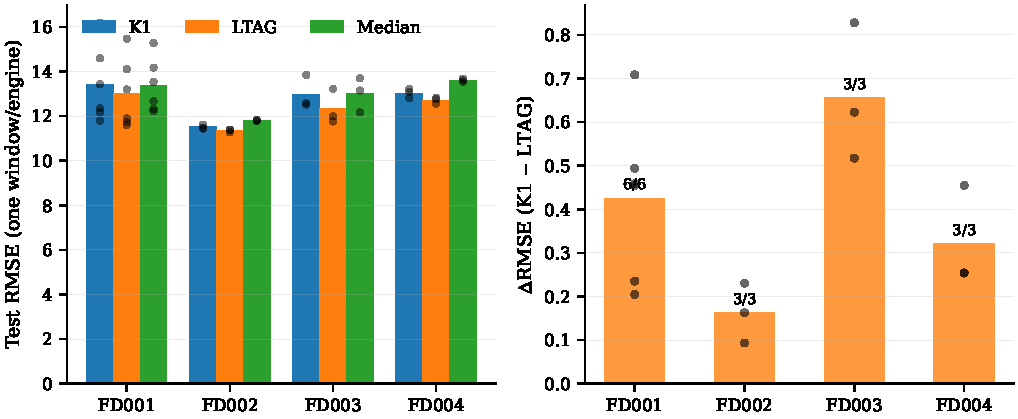
\includegraphics[width=0.48\textwidth]{fig2_test.pdf}
\caption{Frozen B0 test RMSE (one window per engine). Bars are subset means; dots
are individual seeds. LTAG is lower than K1 on all four subsets (15/15).}
\label{fig:test}
\end{figure}

\subsection{Ensemble control}

Averaging three seeds (101/202/303) gives Ens3-K1 11.005/11.231/11.828/13.342 and
Ens3-LTAG 10.292/10.937/11.410/13.228. The gate still helps on top of the
ensemble (4/4), but the ensemble itself closes much of the gap. Ens3-LTAG remains
below LS-ctx on all four subsets (9.256/10.483/11.026/12.903), so the ensemble
control does not rescue the gate as a universal aggregator.
